% TikZ scaffold + photo frames. Photos in Figures/intro_frames/ are LOW-RES CROPS of
% the old simple.png -- replace each file with the original high-res photo (same
% filename) and the figure updates automatically.
\resizebox{\textwidth}{!}{%
\begin{tikzpicture}[font=\small,
  photo/.style={inner sep=0pt, outer sep=0pt},
  quote/.style={font=\scriptsize\itshape, text depth=0pt},
  banner/.style={font=\small\bfseries, anchor=west},
]
% ---------- (1) Teach ----------
\node[photo] (t1) {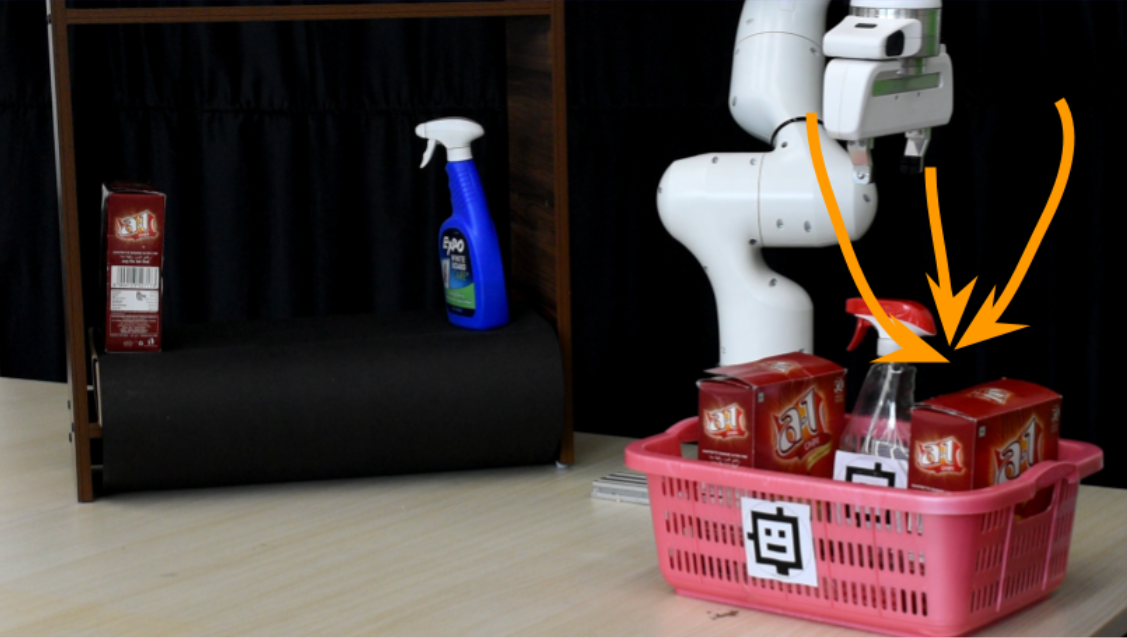
\includegraphics[width=3.1cm]{Figures/intro_frames/teach1.png}};
\node[photo, right=1.5mm of t1] (t2) {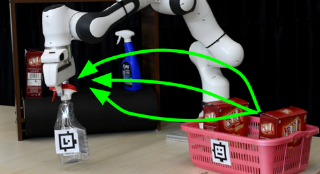
\includegraphics[width=3.1cm]{Figures/intro_frames/teach2.png}};
\node[photo, right=1.5mm of t2] (t3) {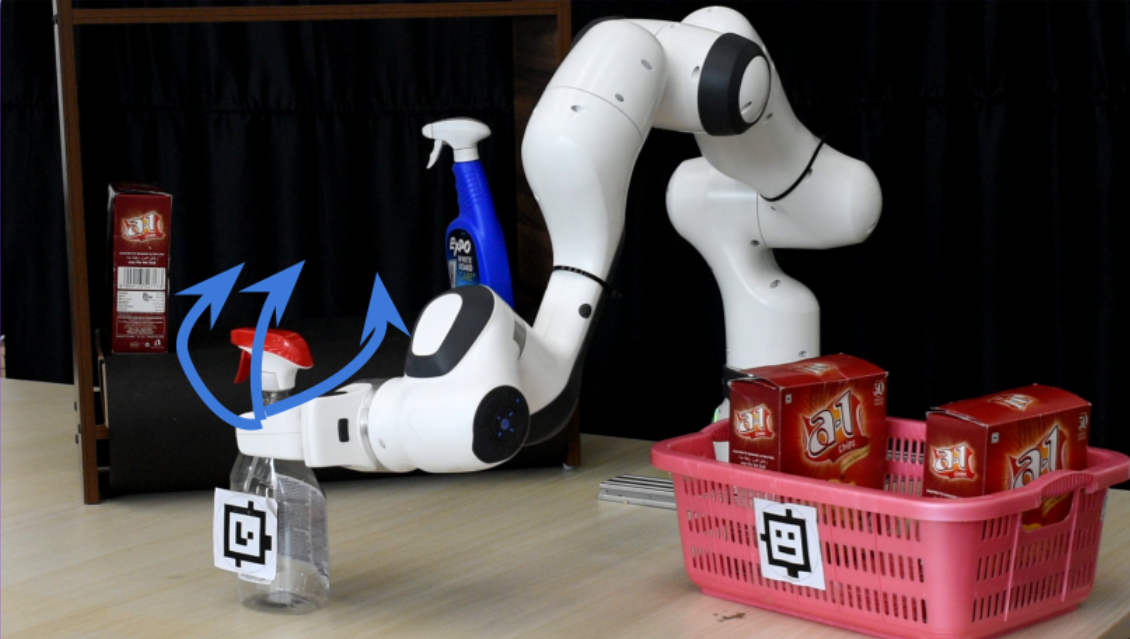
\includegraphics[width=3.1cm]{Figures/intro_frames/teach3.png}};
\node[photo, right=1.5mm of t3] (t4) {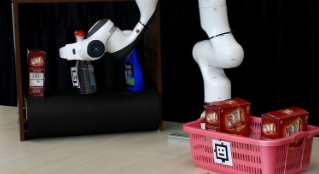
\includegraphics[width=3.1cm]{Figures/intro_frames/teach4.png}};
\node[quote, below=0.5mm of t1] {``grasping from top''};
\node[quote, below=0.5mm of t2] {``placing on table''};
\node[quote, below=0.5mm of t3] {``grasping from side''};
\node[quote, below=0.5mm of t4] {``placing on shelf''};
\node[banner, tli] at ([xshift=-1mm,yshift=3.5mm]t1.north west)
  {\faUser~1.\ Expert teaches: narrated, segmented demonstrations};
\begin{scope}[on background layer]
  \node[fill=teachbg, rounded corners, inner sep=2.5mm,
        fit=(t1)(t4), yshift=-1mm, minimum height=2.6cm] (teachbox) {};
\end{scope}
% ---------- (2) Query ----------
\node[photo, below=13mm of t1.south west, anchor=north west] (q1a)
  {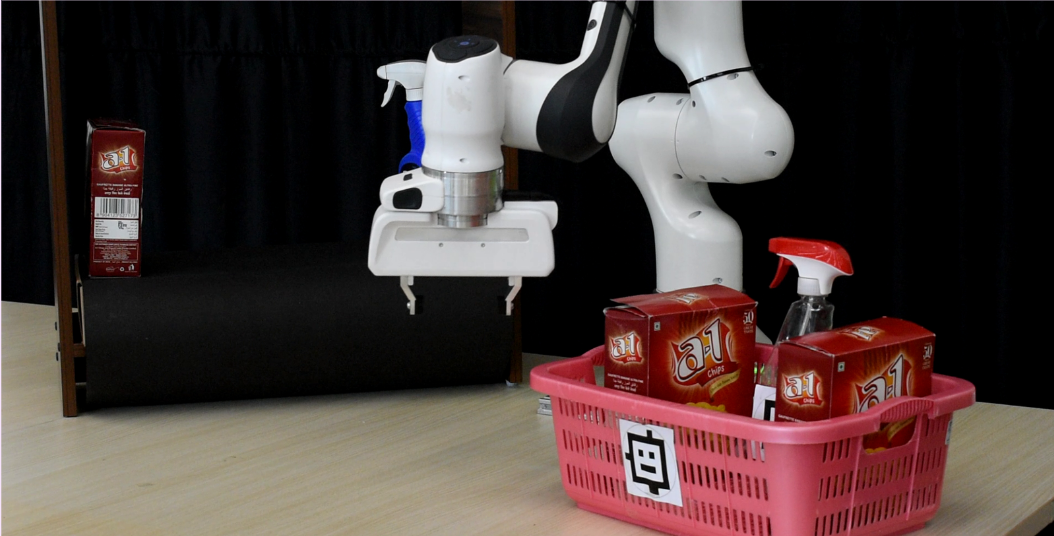
\includegraphics[width=2.75cm]{Figures/intro_frames/query1a.png}};
\node[photo, right=4mm of q1a] (q1b) {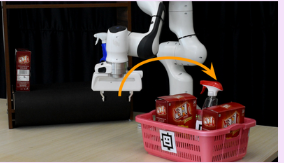
\includegraphics[width=2.75cm]{Figures/intro_frames/query1b.png}};
\node[photo, right=7mm of q1b] (q2a) {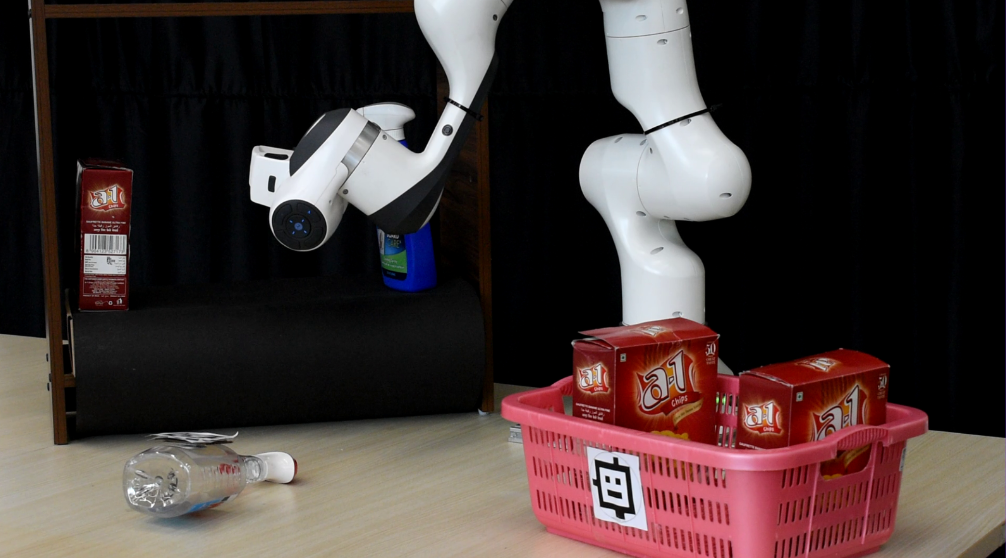
\includegraphics[width=2.75cm]{Figures/intro_frames/query2a.png}};
\node[photo, right=4mm of q2a] (q2b) {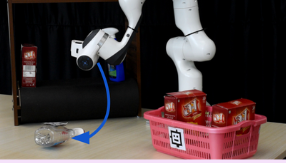
\includegraphics[width=2.75cm]{Figures/intro_frames/query2b.png}};
\draw[->, thick] (q1a) -- (q1b);
\draw[->, thick] (q2a) -- (q2b);
\node[quote, below=0.5mm of q1b.south west, anchor=north] at ([xshift=-3mm]q1b.south west|-q1b.south)
  {};
\node[quote] at ([yshift=-2.5mm]$(q1a.south)!0.5!(q1b.south)$) {\faUser~``I would grasp from top''};
\node[quote] at ([yshift=-2.5mm]$(q2a.south)!0.5!(q2b.south)$) {\faUser~``I would grasp from side''};
\node[banner, tli] at ([xshift=-1mm,yshift=3.5mm]q1a.north west)
  {\faRobot~2.\ Robot queries the situations it is uncertain about};
\begin{scope}[on background layer]
  \node[fill=querybg, rounded corners, inner sep=2.5mm,
        fit=(q1a)(q2b), yshift=-1mm, minimum height=2.6cm] (querybox) {};
\end{scope}
% ---------- (3) Test ----------
\node[photo, right=8mm of t4.north east, anchor=north west, yshift=-9mm] (test)
  {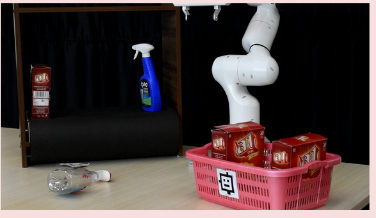
\includegraphics[width=4.1cm]{Figures/intro_frames/test.png}};
\node[banner, tli, text width=4.1cm, align=left] at ([xshift=-1mm,yshift=6mm]test.north west)
  {\faBolt~3.\ Test: perturbation};
\node[font=\scriptsize, align=center, below=1.5mm of test]
  (testtxt) {bottle knocked over $\rightarrow$ localizer\\ detects mode change $\rightarrow$\\ ``grasp from side'' engaged\\ \textbf{failure avoided}};
\begin{scope}[on background layer]
  \node[fill=testbg, rounded corners, inner sep=2.5mm, fit=(test)(testtxt)] {};
\end{scope}
\end{tikzpicture}%
}
